\documentclass[11pt,a4paper]{article}
\usepackage[utf8]{inputenc}\usepackage[T1]{fontenc}\usepackage{lmodern}
\usepackage[margin=2.3cm]{geometry}
\usepackage{amsmath,booktabs,tabularx,longtable,graphicx,float,xcolor,enumitem,caption,fancyhdr,titlesec,listings}
\usepackage[hidelinks]{hyperref}
\definecolor{udblue}{RGB}{31,58,95}
\titleformat{\section}{\Large\bfseries\color{udblue}}{\thesection}{0.8em}{}
\titleformat{\subsection}{\large\bfseries\color{udblue}}{\thesubsection}{0.8em}{}
\pagestyle{fancy}\fancyhf{}
\fancyhead[L]{\small\color{udblue}\textbf{Workshop \#3 Technical Report} \textcolor{gray}{$|$ Landslide Monitoring Colombia}}
\fancyfoot[C]{\thepage}\renewcommand{\headrulewidth}{0.4pt}
\lstset{basicstyle=\ttfamily\footnotesize,breaklines=true,frame=single,backgroundcolor=\color{gray!6},columns=fullflexible}
\captionsetup{font=small,labelfont=bf}
\setlist{itemsep=2pt,topsep=3pt}
\renewcommand{\arraystretch}{1.15}
\newcolumntype{L}{>{\raggedright\arraybackslash}X}
\begin{document}
\thispagestyle{empty}
\begin{center}
{\large\bfseries UNIVERSIDAD DISTRITAL FRANCISCO JOSÉ DE CALDAS}\\
Faculty of Engineering --- Systems Engineering\\[0.4em]
\textsc{Programming for Data Analysis --- Semester 2026-II}\\
\textit{Professor: Carlos Andrés Sierra, M.Sc.}\\[2em]
{\LARGE\color{udblue} Workshop No. 3: Silver-to-Gold Pipeline, Governance KPIs, and Storytelling Definition}\\[1em]
{\large\bfseries Distributed Gold-Layer Analytics with PySpark for Rainfall-Triggered Landslide Risk Monitoring in Colombia}\\[1.2em]
{\bfseries Team 7}\\[1em]
\textbf{Samuel Alberto Leal Saenz} --- Cod. 20231020072\\
\textbf{Cristian Andres Gamez Nuñez} --- Cod. 20231020100\\
\textbf{Sara Nicolle Martinez Moreno} --- Cod. 20231020116\\[0.6em]
{\small GitHub Repository: \url{https://github.com/saritxm/landslide-monitoring-colombia.git}}\\[1em]
November 2026
\end{center}
\vspace{1em}
\begin{abstract}
This report documents the third phase of the landslide risk monitoring platform for Colombia. Building on the Bronze
ingestion and FileSensor-triggered Silver layers delivered in Workshop \#2, we (i) revise both pipelines using the
evidence produced by real runs in development and in the Docker Compose stack, and (ii) implement the Gold layer of the
Medallion Architecture. A scheduled Airflow DAG runs PySpark in local mode, reads each Silver topic folder as a single
distributed DataFrame and persists two Parquet summaries: a governance dataset with 138 data-quality KPI records
and a storytelling dataset with 1,789 analytical records organized in 13 dashboard-ready sections. Twelve
data-quality findings, measured over 9 Silver files, justify every governance KPI. The storytelling layer
operationalizes the Landslide Risk Indicator (LRI) defined in Workshop \#1 for ten Andean monitoring points, contrasts
current rainfall with a ten-year ERA5 baseline, and links each point to its documented landslide history and to the
vocabulary of the NASA catalog narratives. In the latest run, 1 point is classified MEDIUM
and 9 LOW; the highest score corresponds to Pasto (0.51), where five-day
rainfall reaches 99% of the November 90th percentile.
\end{abstract}
\noindent\textbf{Keywords:} Medallion Architecture, PySpark, Apache Airflow, Data Governance, Data Quality KPIs,
Storytelling, Landslide Risk Indicator, Colombia.
\newpage
\tableofcontents
\newpage

\section{Executive Summary}
Workshop \#3 has two goals. The first is to \textbf{improve the Bronze and Silver pipelines} with what the real runs of
Workshop \#2 revealed; nine improvements are documented with a before/after comparison in Section~\ref{sec:improve}.
The second is the \textbf{Gold layer}: the DAG \texttt{gold\_\allowbreak{}processing\_\allowbreak{}dag} reads all accumulated Silver Parquet files with
PySpark and writes:
\begin{itemize}
\item \texttt{governance\_\allowbreak{}20261121\_\allowbreak{}175940.\allowbreak{}parquet}: governance KPIs (null rate per field, volume, duplicate rate, schema compliance, outlier and
quality-flag rates, text statistics, language share, ingestion compliance, freshness and anomalous station-years) for the
data-platform user story US-06.
\item \texttt{storytelling\_\allowbreak{}20261121\_\allowbreak{}175940.\allowbreak{}parquet}: analytical aggregations for the functional dashboard (US-01 to US-04): LRI per monitoring
point, risk-level distribution, hourly and daily rainfall against history, monthly climatology, historical landslides by
year, trigger, size and department, events within 30~km of each point, keywords and bigrams.
\end{itemize}
\paragraph{Adapting the statement to the hazard.} The workshop statement is phrased for opinion mining. In this project
the role of the sentiment label is played by the \textbf{risk level} (LOW/MEDIUM/HIGH) of the LRI, the opinion trend
by the \textbf{rainfall trend relative to its historical percentile}, the keyword--sentiment association by the
\textbf{mean fatalities of the events whose narrative contains each keyword}, and the text corpus by the NASA Global
Landslide Catalog narratives.

\section{Pipeline Improvements Based on Experimentation}\label{sec:improve}
Table~\ref{tab:improve} lists every change made to Bronze, Silver and the infrastructure. Several were discovered only
when the first Spark job was executed, which is the experimentation process the workshop asks to document.
\begin{longtable}{p{4.1cm}p{3.0cm}p{4.6cm}p{3.4cm}}
\caption{Before/after comparison of pipeline improvements}\label{tab:improve}\\\toprule
\textbf{Observation} & \textbf{Before} & \textbf{After (Workshop \#3)} & \textbf{Reason}\\\midrule\endfirsthead
\toprule\textbf{Observation} & \textbf{Before} & \textbf{After} & \textbf{Reason}\\\midrule\endhead
Four Silver topics with different schemas share one folder, so \texttt{spark.\allowbreak{}read.\allowbreak{}parquet(\allowbreak{}"datalake\_\allowbreak{}silver/\allowbreak{}")} cannot produce one DataFrame &
All files in \texttt{datalake\_\allowbreak{}silver/\allowbreak{}} & One sub-folder per topic, created by the writer; \texttt{scripts/\allowbreak{}migrate\_\allowbreak{}silver\_\allowbreak{}w3.\allowbreak{}py} moved existing files &
Each folder has one consistent schema (cloud-folder read pattern)\\
Spark 3.5 error \textit{Illegal Parquet type: TIMESTAMP(NANOS)} & pandas wrote nanosecond timestamps &
Writer forces microseconds (\texttt{coerce\_\allowbreak{}timestamps='us'}); existing files converted without loss & Sources have at most second precision\\
88.9\% of rainfall rows repeat a station-hour; 36.5\% of repeated hours change value between polls &
Every poll stored & Gold keeps the most recent poll per station-hour (window \texttt{row\_\allowbreak{}number}) & Open-Meteo revises the past two days\\
ERA5 7-day sums null at every year boundary (600 rows) & Rolling sum per yearly file & Rolling sums recomputed in Gold across years & Antecedent rain spans New Year\\
Implausible ERA5 annual totals: Pereira 2016 (14,499 mm), Manizales 2016 (17,122 mm) & Documented only & Station-years above $2\times$ the station median flagged and excluded from percentiles & They would inflate the P90 baseline\\
Generic words dominate GLC tokens (\textit{said} 83, \textit{two} 52, \textit{least} 43) & EN+ES stop words & Domain noise list in \texttt{nlp.\allowbreak{}py} and Gold; bigrams added & Keywords must describe events\\
Timestamps collected from Spark shifted by $-5$~h & Python \texttt{collect(\allowbreak{})} converts to local time & Time arithmetic and formatting inside Spark (session zone UTC) & Freshness KPIs were wrong\\
Spark workers failed (Python version mismatch) & Default interpreter & \texttt{PYSPARK\_\allowbreak{}PYTHON} pinned to the task interpreter & Driver and workers must match\\
No Java in the Airflow image & Airflow 2.9.2 + libraries & OpenJDK 17 and \texttt{pyspark==3.\allowbreak{}5.\allowbreak{}3} in the Dockerfile; \texttt{SPARK\_\allowbreak{}DRIVER\_\allowbreak{}MEMORY} in compose & PySpark needs a JVM\\
\bottomrule
\end{longtable}
Bronze reliability improvements made during the Workshop \#2 revision remain in force: retries and execution timeouts,
no offline fallback that could write invented data, and skipping of unchanged payloads.

\section{Data Quality Findings in the Silver Layer}
The findings were measured with pandas in \texttt{notebooks/\allowbreak{}03\_\allowbreak{}data\_\allowbreak{}quality\_\allowbreak{}findings.\allowbreak{}ipynb} and, independently, with PySpark
in the governance dataset. Silver currently holds 9 Parquet files (rainfall: 6, rainfall\_historical: 1, landslides: 1, lhasa\_hazard: 1).
\begin{longtable}{p{0.4cm}p{3.6cm}p{3.4cm}p{4.0cm}p{3.4cm}}
\caption{Data-quality findings and handling strategy}\label{tab:findings}\\\toprule
\textbf{\#} & \textbf{Field} & \textbf{Issue} & \textbf{Frequency / severity} & \textbf{Handling}\\\midrule\endfirsthead
\toprule\textbf{\#} & \textbf{Field} & \textbf{Issue} & \textbf{Frequency} & \textbf{Handling}\\\midrule\endhead
F1 & rainfall: station + hour & Duplicates across polls, revised values & 88.9\% repeated keys & Latest poll kept\\
F2 & landslides: event time & 00:00 means unknown time & 64.2\% of events & Flag; daily resolution\\
F3 & landslides: \texttt{country\_\allowbreak{}name} & Null inside the Colombia box (Mocoa 2017) & 7.3\% & Kept null + flag\\
F4 & landslides: fatality / injury counts & Unknown counts & 4.6\% / 74.3\% null & Kept null (never 0)\\
F5 & landslides: \texttt{event\_\allowbreak{}time}, \texttt{storm\_\allowbreak{}name}, \texttt{notes}, \texttt{photo\_\allowbreak{}link} & Empty columns & 100 / 100 / 98 / 87\% null & Not used; monitored\\
F6 & landslides: fatalities & Extreme values & 6.4\% IQR flags (max 329, Mocoa) & Flagged, not removed\\
F7 & rainfall: precipitation & Convective extremes & 3.9\% IQR, 1.2\% Z flags & Per-station, wet hours\\
F8 & ERA5 annual totals & Reanalysis anomaly & 2 station-years $>2\times$ median & Excluded from percentiles\\
F9 & ERA5 \texttt{precip\_\allowbreak{}7d\_\allowbreak{}mm} & Nulls at year boundaries & 1.64\% & Recomputed in Gold\\
F10 & rainfall ingestion & Missing hourly polls & 42\% (5 of 12 expected hourly polls between 2026-11-21 06:40 and 2026-11-21 17:23 UTC) & Compliance KPI\\
F11 & GLC narratives & Length and language & mean 568 chars (min 71, max 1264); 96.3\% English & Text KPIs; EN+ES stop words\\
F12 & LHASA & One raster per day; only the newest kept & 10 station windows & Daily cadence; freshness\\
\bottomrule
\end{longtable}
\begin{figure}[H]\centering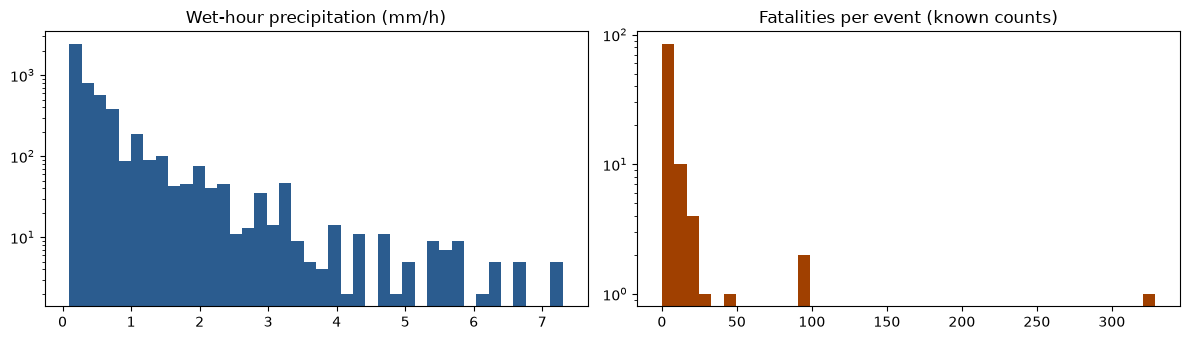
\includegraphics[width=0.92\textwidth]{../img/dq_findings.png}
\caption{Distribution of wet-hour precipitation and of known fatalities per event (log scale). The tails contain the values flagged by the IQR and Z-score rules (F6, F7).}\end{figure}
\begin{longtable}{p{2.6cm}p{4.6cm}p{1.6cm}p{5.6cm}}
\caption{Fields with a non-zero null rate (PySpark governance KPI \texttt{null\_\allowbreak{}rate})}\\\toprule
\textbf{Topic} & \textbf{Field} & \textbf{Null \%} & \textbf{Detail}\\\midrule\endfirsthead
\toprule\textbf{Topic} & \textbf{Field} & \textbf{Null \%} & \textbf{Detail}\\\midrule\endhead
landslides & \texttt{event\_\allowbreak{}time} & 100.00 & 109 of 109 \\
landslides & \texttt{storm\_\allowbreak{}name} & 100.00 & 109 of 109 \\
landslides & \texttt{notes} & 98.17 & 107 of 109 \\
landslides & \texttt{photo\_\allowbreak{}link} & 87.16 & 95 of 109 \\
landslides & \texttt{injury\_\allowbreak{}count} & 74.31 & 81 of 109 \\
landslides & \texttt{country\_\allowbreak{}name} & 7.34 & 8 of 109 \\
landslides & \texttt{event\_\allowbreak{}import\_\allowbreak{}source} & 7.34 & 8 of 109 \\
landslides & \texttt{event\_\allowbreak{}import\_\allowbreak{}id} & 7.34 & 8 of 109 \\
landslides & \texttt{country\_\allowbreak{}code} & 7.34 & 8 of 109 \\
landslides & \texttt{admin\_\allowbreak{}division\_\allowbreak{}population} & 7.34 & 8 of 109 \\
landslides & \texttt{gazeteer\_\allowbreak{}closest\_\allowbreak{}point} & 7.34 & 8 of 109 \\
landslides & \texttt{gazeteer\_\allowbreak{}distance} & 7.34 & 8 of 109 \\
landslides & \texttt{fatality\_\allowbreak{}count} & 4.59 & 5 of 109 \\
rainfall\_historical & \texttt{precip\_\allowbreak{}7d\_\allowbreak{}mm} & 1.64 & 600 of 36530 \\
landslides & \texttt{event\_\allowbreak{}description} & 0.92 & 1 of 109 \\
landslides & \texttt{landslide\_\allowbreak{}setting} & 0.92 & 1 of 109 \\
\bottomrule\end{longtable}

\section{Governance KPI Definition}
The governance dataset is a long table with schema
(\texttt{kpi}, \texttt{topic}, \texttt{field}, \texttt{period}, \texttt{value}, \texttt{unit}, \texttt{detail}, \texttt{computed\_\allowbreak{}at\_\allowbreak{}utc}),
so the governance dashboard (US-06) selects each KPI with a filter. For a topic with $N$ rows:
\begin{align}
\text{NullRate}(f) &= \frac{100}{N}\sum_{i=1}^{N} \mathbf{1}[x_{i,f} = \text{null} \lor x_{i,f} = \text{''}] &
\text{DupRate} &= 100\cdot\frac{N - |\{\text{distinct natural keys}\}|}{N}\\
\text{Compliance} &= \frac{100}{N}\sum_{i} \mathbf{1}[\text{required}(i)\land \text{bounds}(i)] &
\text{IngestionCompliance} &= 100\cdot\frac{\text{hours with a poll}}{\text{hours in the observed window}}
\end{align}
\begin{small}\begin{longtable}{p{3.6cm}p{4.9cm}p{2.4cm}p{3.9cm}}
\caption{Governance KPIs, computation and justification}\\\toprule
\textbf{KPI} & \textbf{PySpark computation} & \textbf{Justified by} & \textbf{Latest value}\\\midrule\endfirsthead
\toprule\textbf{KPI} & \textbf{Computation} & \textbf{Justified by} & \textbf{Latest value}\\\midrule\endhead
\texttt{null\_\allowbreak{}rate} & \texttt{sum(\allowbreak{}isNull|empty)} per column $/N$ & F3, F4, F5, F9 & 89 field records\\
\texttt{volume\_\allowbreak{}rows}, \texttt{volume\_\allowbreak{}bronze\_\allowbreak{}files}, \texttt{volume\_\allowbreak{}rows\_\allowbreak{}per\_\allowbreak{}day} & \texttt{count}, \texttt{countDistinct(\allowbreak{}\_\allowbreak{}bronze\_\allowbreak{}source\_\allowbreak{}file)}, \texttt{groupBy}(processing day) & Volume per source & rainfall 10,800 rows / 9 polls\\
\texttt{duplicate\_\allowbreak{}rate\_\allowbreak{}before}/\texttt{\_\allowbreak{}after} & rows $-$ distinct natural keys & F1 (preventive for GLC/ERA5: 0\%) & rainfall 88.9\% $\to$ 0\%\\
\texttt{schema\_\allowbreak{}compliance\_\allowbreak{}rate} & required fields non-null and inside physical bounds & Silver contract & 100\% for all topics\\
\texttt{outlier\_\allowbreak{}rate} & \texttt{avg(\allowbreak{}flag)} per outlier flag & F6, F7 & precipitation IQR 3.9\%\\
\texttt{flag\_\allowbreak{}rate} & \texttt{avg(\allowbreak{}flag)} per quality flag & F2, F3, F4 & unknown time 64.2\%\\
\texttt{text\_\allowbreak{}length\_\allowbreak{}*} & \texttt{length}: mean, \texttt{percentile\_\allowbreak{}approx(\allowbreak{}0.\allowbreak{}5)}, min, max & F11 & median 577 characters\\
\texttt{language\_\allowbreak{}share} & English vs Spanish marker words (\texttt{array\_\allowbreak{}intersect}) & F11 & es 3.7, en 96.3\%\\
\texttt{ingestion\_\allowbreak{}compliance} & hourly polls present / expected; ERA5 years / 10 & F10 & rainfall 42\%, ERA5 100\%\\
\texttt{freshness\_\allowbreak{}hours} & run time $-$ max(\texttt{\_\allowbreak{}processed\_\allowbreak{}at\_\allowbreak{}utc}) in Spark & US-06 outages & rainfall 0.6~h\\
\texttt{anomalous\_\allowbreak{}station\_\allowbreak{}year} & annual total $> 2\times$ station median & F8 & 2 records\\
\bottomrule\end{longtable}\end{small}

\section{Storytelling Aggregations and Dashboard Narrative}
\subsection{Narrative}
\textit{``Which Andean areas of Colombia are at landslide risk right now, and is the rain falling there unusual for this
time of year?''} After viewing the dashboard, the UNGRD analyst should know which monitoring points to watch, whether
that is driven by rainfall that is high for the season, and whether those places have a history of deadly landslides.
Each aggregation below maps to one user story of Workshop \#1 and to one dashboard element.
\begin{small}\begin{longtable}{p{3.9cm}p{6.2cm}p{1.6cm}p{2.6cm}}
\caption{Storytelling sections, user stories and dashboard elements}\\\toprule
\textbf{Section (rows)} & \textbf{PySpark aggregation} & \textbf{Story} & \textbf{Dashboard}\\\midrule\endfirsthead
\toprule\textbf{Section} & \textbf{Aggregation} & \textbf{Story} & \textbf{Dashboard}\\\midrule\endhead
\texttt{station\_\allowbreak{}risk} (100) & Latest poll per point; $P_{24h}$, 5-day antecedent rain, November 5-day P90 (ERA5), LHASA P90, events within 30~km; LRI score and level & US-01/02/03 & Risk map and table\\
\texttt{risk\_\allowbreak{}level\_\allowbreak{}distribution} (3) & Points per level (analogue of the sentiment distribution) & US-01 & KPI cards\\
\texttt{hourly\_\allowbreak{}rainfall} (1200) & Hourly series of the latest poll, observed vs forecast & US-02 & Line chart\\
\texttt{daily\_\allowbreak{}rain\_\allowbreak{}vs\_\allowbreak{}history} (50) & Daily totals vs historical daily P90 of the month & US-03 & Bars + threshold\\
\texttt{monthly\_\allowbreak{}climatology} (240) & Mean daily rain and 5-day P90 per point and month & US-03 & Seasonal profile\\
\texttt{landslides\_\allowbreak{}by\_\allowbreak{}*} (90) & Events and known fatalities by year, trigger, size, department & US-04 & Bar charts\\
\texttt{landslides\_\allowbreak{}near\_\allowbreak{}station} (35) & Haversine cross join, distance $\le 30$~km & US-04 & Map layer\\
\texttt{top\_\allowbreak{}keywords} (50), \texttt{top\_\allowbreak{}bigrams} (20) & Frequencies after noise removal; mean fatalities per keyword (keyword--severity association) & US-04 & Word bars\\
\texttt{narrative} (1) & Key-insight sentence generated from the data & US-01 & Header\\
\bottomrule\end{longtable}\end{small}

\subsection{Landslide Risk Indicator in the Gold layer}
For monitoring point $c$ and the latest forecast poll $t$, the LRI of Workshop \#1 is computed as
\begin{equation}
S(c,t) = 0.35\min\!\left(1,\frac{P_{24h}}{75\text{ mm}}\right) + 0.35\min\!\left(1,\frac{P_{5d}}{P^{5d,\text{hist}}_{90}(c,m)}\right)
+ 0.20\,H_{\text{LHASA}}(c) + 0.10\min\!\left(1,\frac{D_{30\text{km}}(c)}{5}\right)
\end{equation}
with LOW $<0.40\le$ MEDIUM $<0.70\le$ HIGH. Because each forecast poll covers five days (two past and three forecast
days), the antecedent term compares five-day sums on both sides instead of the seven-day sums planned in Workshop \#1;
$P^{5d,\text{hist}}_{90}$ is computed from ERA5 2016--2025 for the same calendar month, excluding anomalous station-years.

\subsection{Results of the latest run (2026-11-21 12:23 UTC)}
\begin{table}[H]\centering\small
\caption{LRI per monitoring point (LOW: 9, MEDIUM: 1, HIGH: 0)}
\begin{tabular}{lcrrrrrrrr}\toprule
Point & Level & $S$ & $P_{24h}$ & $P_{5d}$ & P90 & ratio & $H$ & $D_{30}$ & deaths\\\midrule
Pasto & MEDIUM & 0.51 & 16.1 & 107.2 & 108.8 & 0.99 & 0.16 & 3 & 14 \\
Medellin & LOW & 0.35 & 11.0 & 31.3 & 61.3 & 0.51 & 0.11 & 9 & 157 \\
Bogota & LOW & 0.26 & 3.2 & 19.7 & 43.1 & 0.46 & 0.01 & 4 & 13 \\
Manizales & LOW & 0.24 & 4.3 & 31.9 & 96.3 & 0.33 & 0.03 & 7 & 94 \\
Ibague & LOW & 0.20 & 7.5 & 47.1 & 99.9 & 0.47 & 0.02 & 0 & -- \\
Cali & LOW & 0.20 & 3.4 & 26.4 & 105.7 & 0.25 & 0.07 & 4 & 6 \\
Bucaramanga & LOW & 0.18 & 2.9 & 19.7 & 111.9 & 0.18 & 0.01 & 5 & 9 \\
Pereira & LOW & 0.17 & 1.4 & 31.7 & 93.4 & 0.34 & 0.01 & 2 & 13 \\
Mocoa & LOW & 0.12 & 4.7 & 22.7 & 107.8 & 0.21 & 0.02 & 1 & 329 \\
Villavicencio & LOW & 0.05 & 1.1 & 8.5 & 77.3 & 0.11 & 0.01 & 0 & -- \\
\bottomrule\end{tabular}\end{table}
\noindent\textbf{Key insight.} Latest forecast (2026-11-21 12:23 UTC): 10 monitoring points; highest risk at Pasto (score 0.51, MEDIUM). Rain relative to history is highest at Pasto: 107 mm in 5 days = 99\% of the November 5-day P90 (109 mm).
\begin{table}[H]\centering\small
\begin{minipage}{0.48\textwidth}\centering
\caption{Top keywords and mean fatalities}\begin{tabular}{lrr}\toprule Keyword & Freq. & Mean deaths\\\midrule
people & 108 & 12.3 \\
landslide & 103 & 13.5 \\
rains & 61 & 5.3 \\
mudslide & 56 & 4.9 \\
heavy & 53 & 18.2 \\
killed & 51 & 10.5 \\
santander & 41 & 3.2 \\
caldas & 38 & 9.8 \\
buried & 38 & 9.3 \\
road & 38 & 3.8 \\
\bottomrule\end{tabular}\end{minipage}\hfill
\begin{minipage}{0.42\textwidth}\centering
\caption{Top bigrams}\begin{tabular}{lr}\toprule Bigram & Freq.\\\midrule
heavy rains & 37 \\
people killed & 14 \\
people dead & 13 \\
rainy season & 12 \\
santa marta & 12 \\
took place & 12 \\
year old & 12 \\
landslide hit & 10 \\
people died & 10 \\
torrential rains & 10 \\
\bottomrule\end{tabular}\end{minipage}\end{table}
\begin{figure}[H]\centering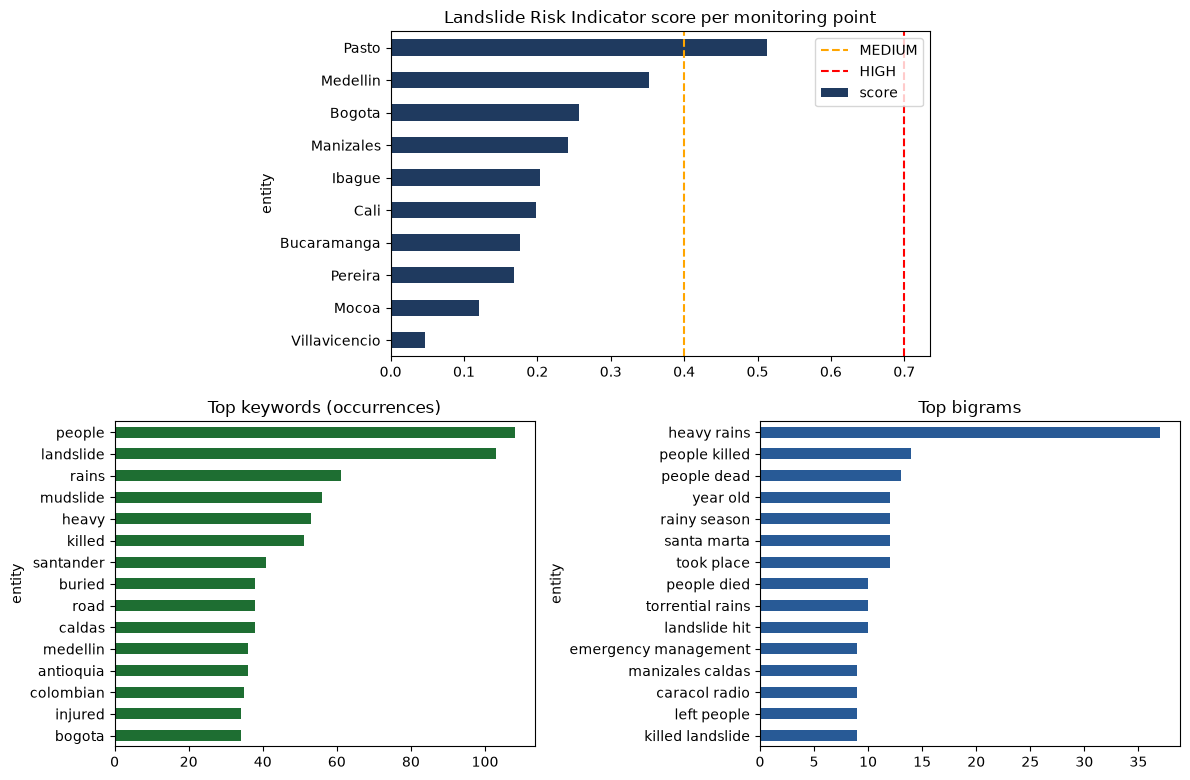
\includegraphics[width=0.9\textwidth]{../img/gold_risk.png}
\caption{Gold preview notebook: LRI score per monitoring point with the MEDIUM and HIGH thresholds, and keyword/bigram distributions read from the storytelling file.}\end{figure}

\section{PySpark Implementation}
\subsection{Spark session}
\begin{lstlisting}[language=Python]
SparkSession.builder.master("local[*]").appName("landslide-gold")
    .config("spark.driver.memory", os.environ.get("SPARK_DRIVER_MEMORY", "1g"))
    .config("spark.sql.shuffle.partitions", "4")
    .config("spark.sql.session.timeZone", "UTC")
    .config("spark.ui.enabled", "false")
    .config("spark.sql.parquet.mergeSchema", "true").getOrCreate()
# PYSPARK_PYTHON / PYSPARK_DRIVER_PYTHON = sys.executable (same interpreter as the task)
\end{lstlisting}
\subsection{DAG structure}
\texttt{gold\_\allowbreak{}processing\_\allowbreak{}dag} (TaskFlow API) runs daily at 00:30~UTC with \texttt{catchup=False}, one retry and a 30-minute
timeout: \texttt{check\_\allowbreak{}silver\_\allowbreak{}inputs} (fails early if a topic folder is empty) $\rightarrow$ \texttt{build\_\allowbreak{}gold} (Spark job)
$\rightarrow$ \texttt{validate\_\allowbreak{}gold} (both files exist and are non-empty).
\subsection{Key transformations}
\begin{itemize}
\item \textbf{Reading:} \texttt{spark.\allowbreak{}read.\allowbreak{}parquet(\allowbreak{}"datalake\_\allowbreak{}silver/\allowbreak{}<topic>/\allowbreak{}")} --- all accumulated files of a topic as one DataFrame.
\item \textbf{Deduplication:} \texttt{row\_\allowbreak{}number(\allowbreak{})} over \texttt{partitionBy(\allowbreak{}station, hour).\allowbreak{}orderBy(\allowbreak{}poll\_\allowbreak{}time desc)}.
\item \textbf{Antecedent rainfall:} window sums across years; \texttt{percentile\_\allowbreak{}approx} for the P90 baselines.
\item \textbf{Spatial join:} cross join of the 10 points with the GLC events and a haversine distance expression.
\item \textbf{Text:} \texttt{filter}, \texttt{explode} and \texttt{transform(\allowbreak{}sequence(\allowbreak{}.\allowbreak{}.\allowbreak{}.\allowbreak{}))} higher-order functions for keywords and bigrams.
\item \textbf{Persistence:} \texttt{unionByName} into the long tables, \texttt{coalesce(\allowbreak{}1).\allowbreak{}write.\allowbreak{}parquet} to a temporary folder,
then the part file is moved to \texttt{datalake\_\allowbreak{}gold/\allowbreak{}<name>\_\allowbreak{}YYYYMMDD\_\allowbreak{}HHMMSS.\allowbreak{}parquet}; existing files are never overwritten.
\end{itemize}
\subsection{Docker adjustments}
The image adds \texttt{openjdk-17-jre-headless} (with \texttt{JAVA\_\allowbreak{}HOME}) and \texttt{pyspark==3.\allowbreak{}5.\allowbreak{}3}; compose sets
\texttt{SPARK\_\allowbreak{}DRIVER\_\allowbreak{}MEMORY=1g} and \texttt{DATALAKE\_\allowbreak{}ROOT}. Local mode needs no extra container; \texttt{datalake\_\allowbreak{}gold/\allowbreak{}} was already mounted.

\section{Results Evidence}
\begin{table}[H]\centering\small\caption{Gold DAG runs}
\begin{tabular}{llll}\toprule Run & Task & State & Seconds\\\midrule
\texttt{scheduled\_\allowbreak{}\_\allowbreak{}2026-11-20T00:30:00+00:00} & check\_silver\_inputs & success & 0.1 \\
\texttt{scheduled\_\allowbreak{}\_\allowbreak{}2026-11-20T00:30:00+00:00} & build\_gold & success & 36.9 \\
\texttt{scheduled\_\allowbreak{}\_\allowbreak{}2026-11-20T00:30:00+00:00} & validate\_gold & success & 0.2 \\
\texttt{manual\_\allowbreak{}\_\allowbreak{}2026-11-21T17:59:40+00:00} & check\_silver\_inputs & success & 0.1 \\
\texttt{manual\_\allowbreak{}\_\allowbreak{}2026-11-21T17:59:40+00:00} & build\_gold & success & 35.9 \\
\texttt{manual\_\allowbreak{}\_\allowbreak{}2026-11-21T17:59:40+00:00} & validate\_gold & success & 0.2 \\
\bottomrule\end{tabular}\end{table}
\noindent The runs were executed with Airflow 2.10.5 on the development machine with the same DAG file; the Docker image
has been updated for PySpark and must be rebuilt (\texttt{docker compose build}) to run the DAG in the containers.
\begin{figure}[H]\centering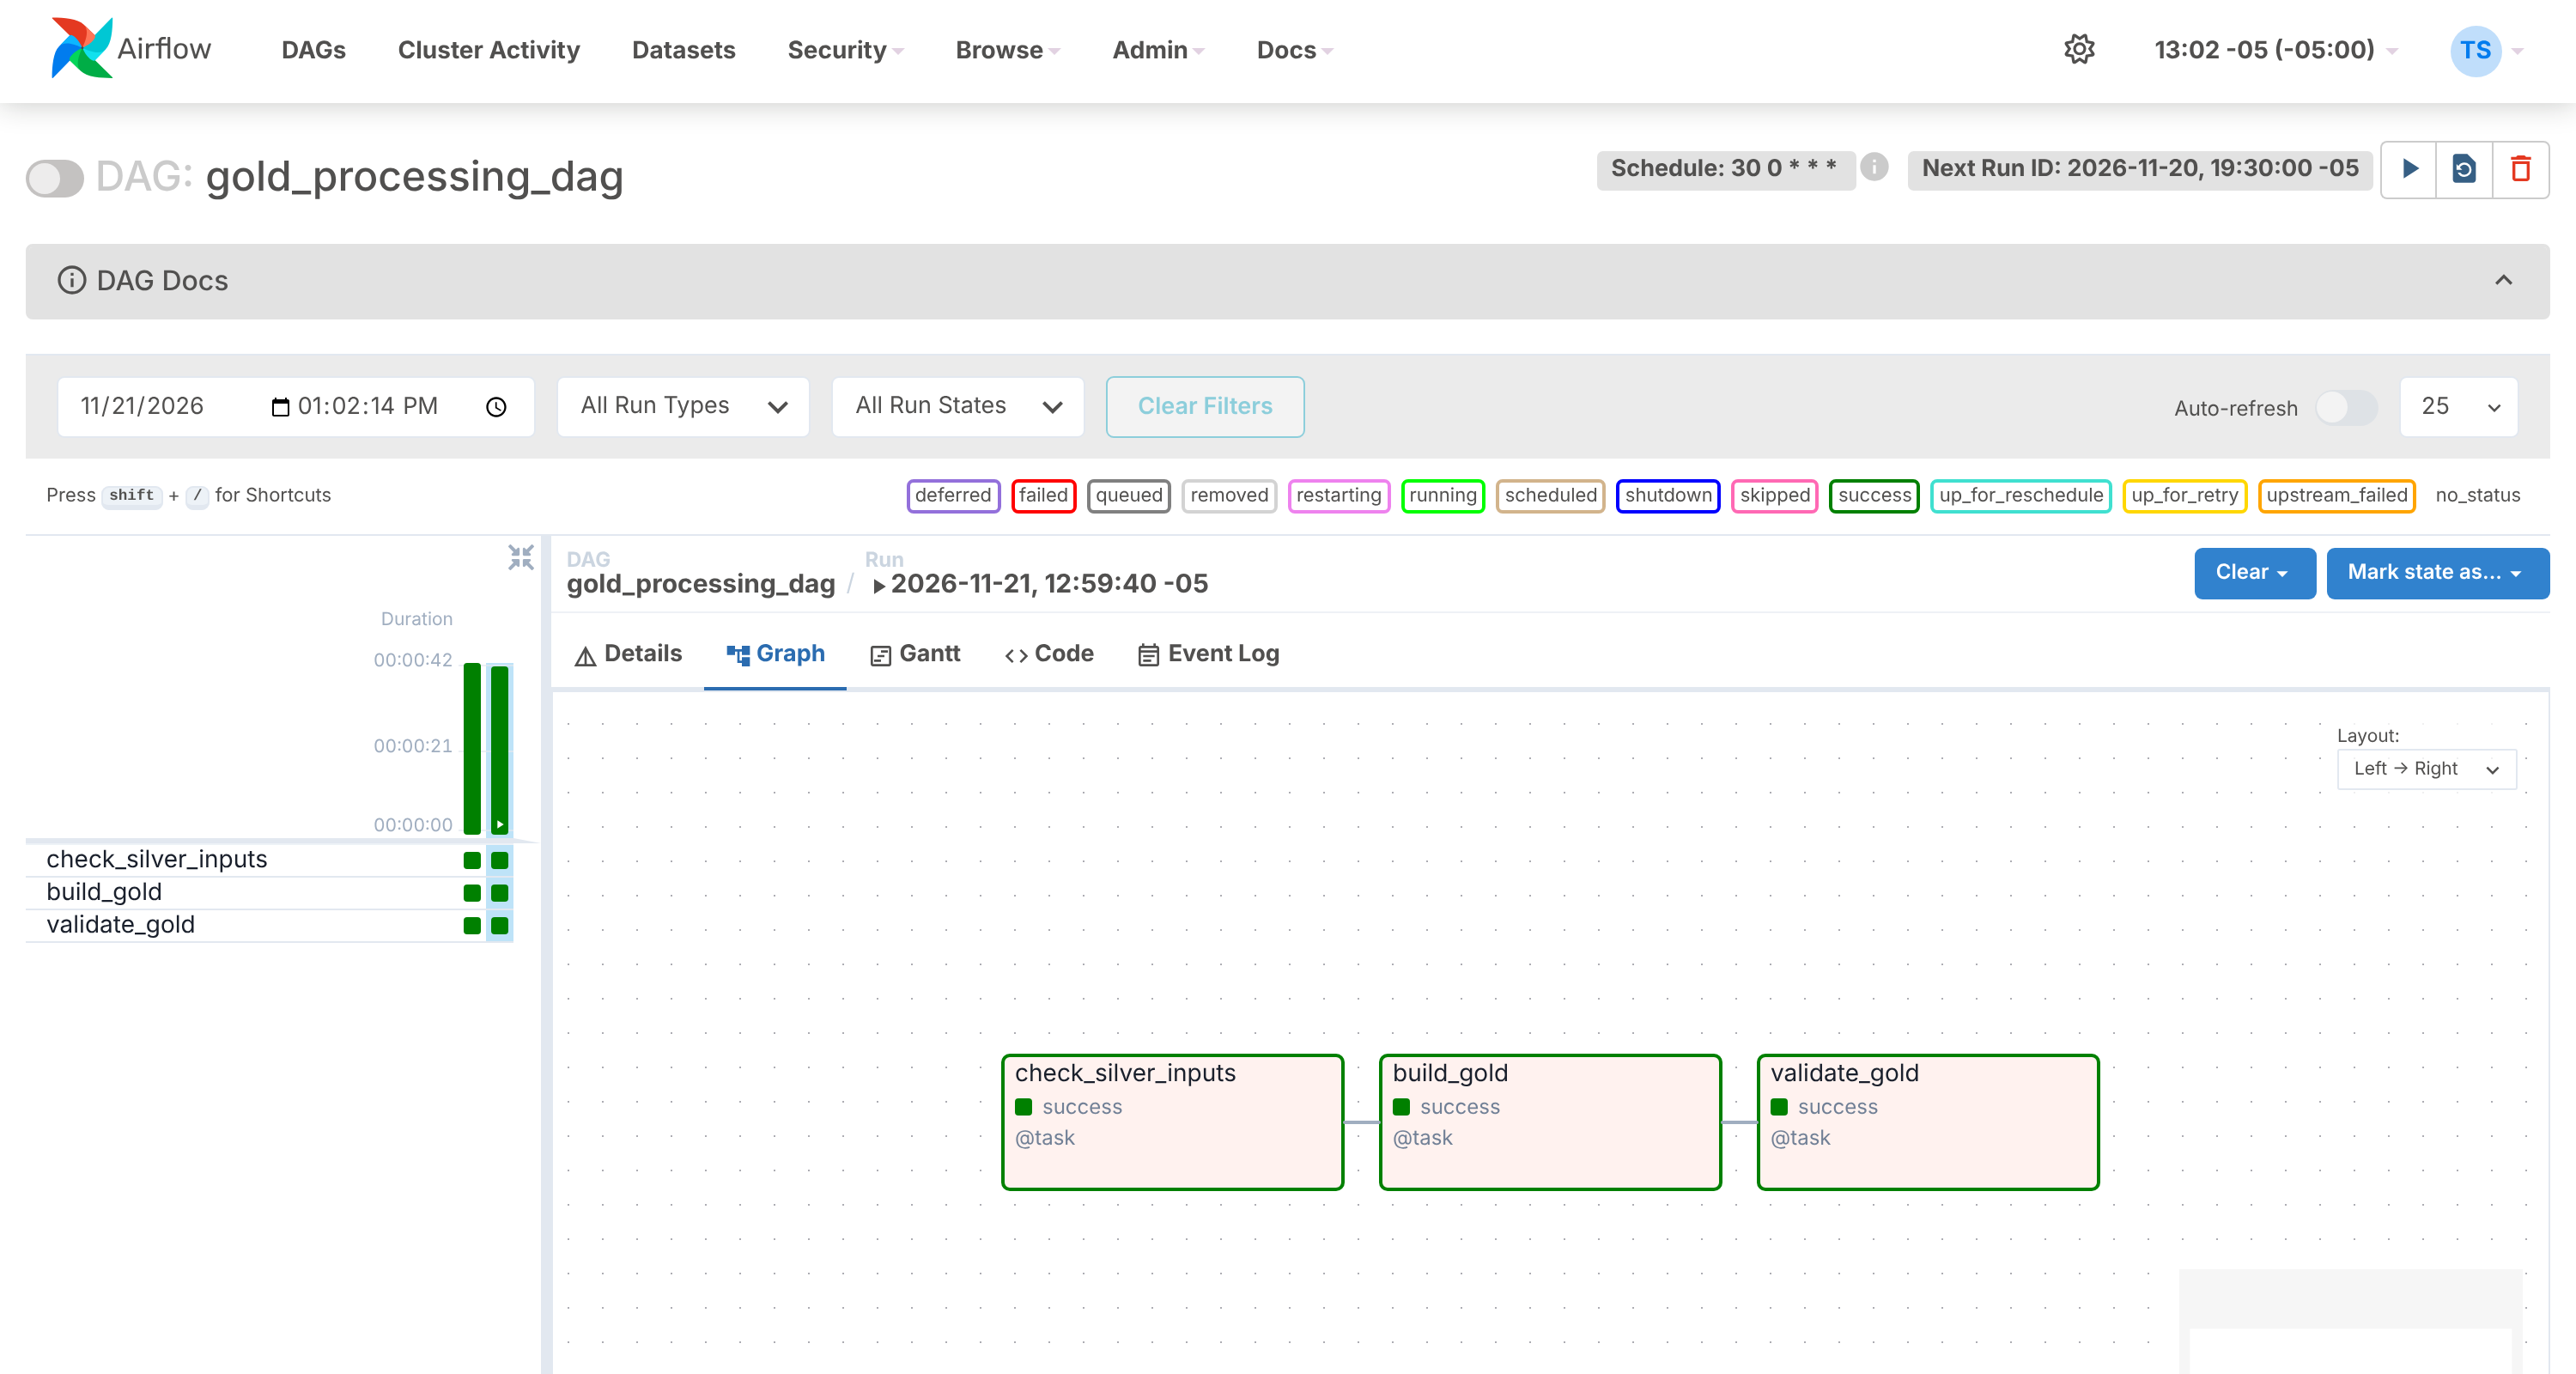
\includegraphics[width=0.9\textwidth]{../img/gold_dag_graph.png}
\caption{\texttt{gold\_\allowbreak{}processing\_\allowbreak{}dag} in the Airflow UI: scheduled and manual runs, all tasks successful.}\end{figure}
\begin{figure}[H]\centering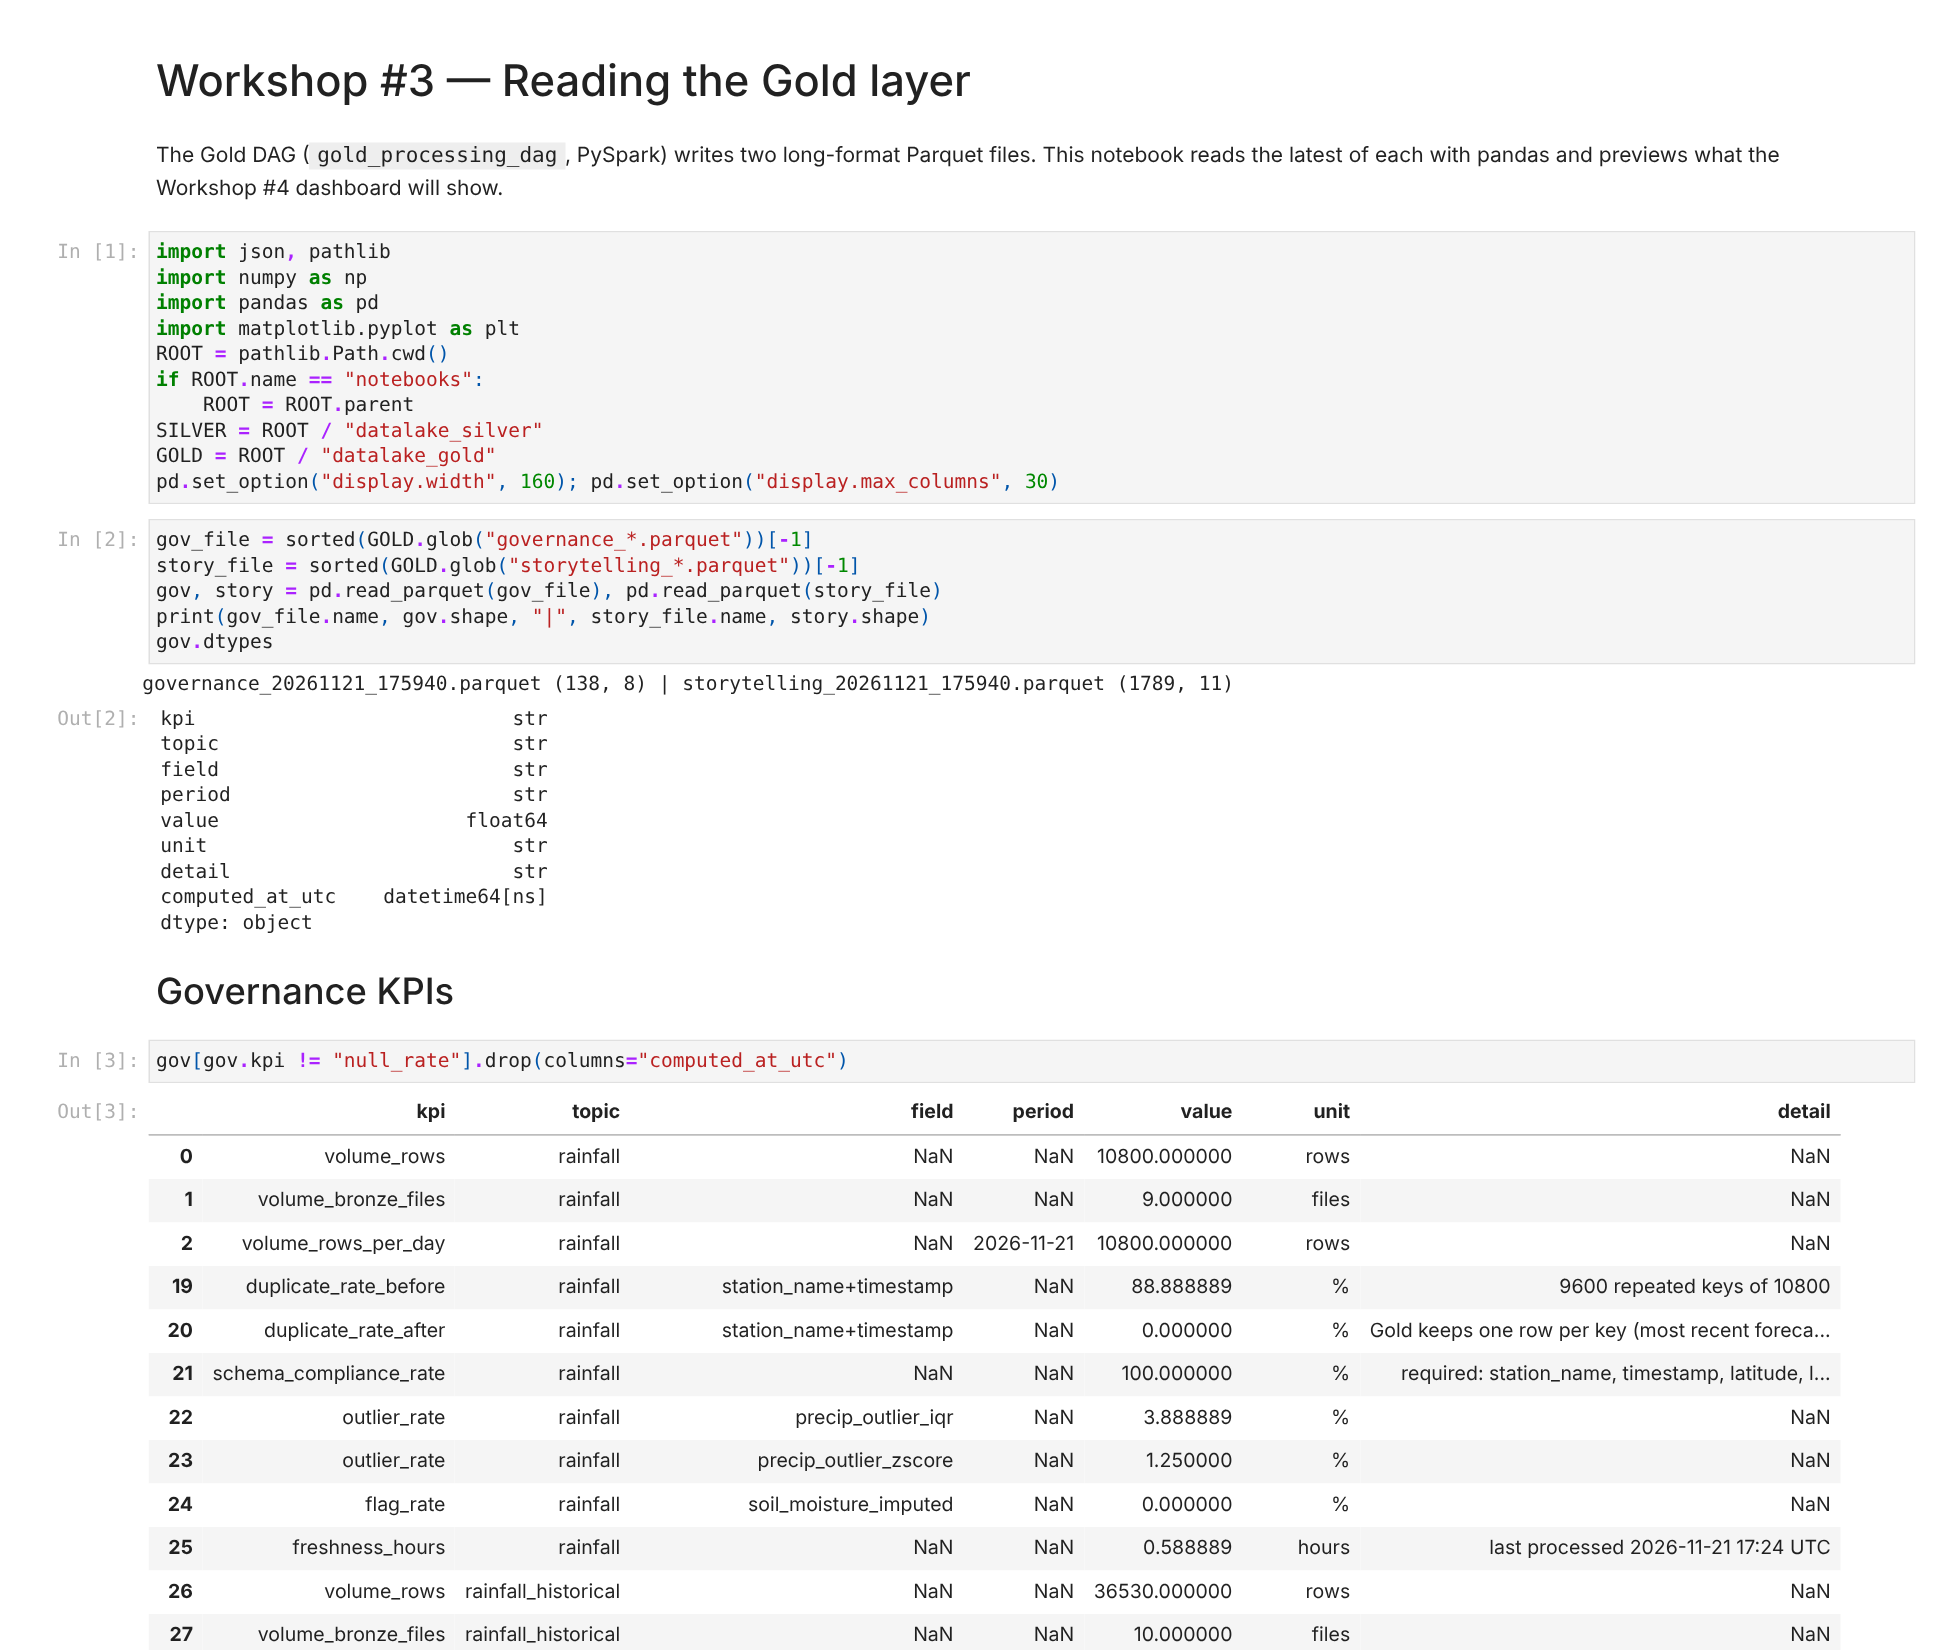
\includegraphics[width=0.85\textwidth]{../img/gold_files.png}
\caption{Governance KPIs read from the Gold Parquet file with pandas (\texttt{notebooks/\allowbreak{}04\_\allowbreak{}gold\_\allowbreak{}preview.\allowbreak{}ipynb}).}\end{figure}
\begin{longtable}{p{4.0cm}p{3.0cm}p{3.8cm}rp{1.4cm}}
\caption{Sample of \texttt{governance\_\allowbreak{}20261121\_\allowbreak{}175940.\allowbreak{}parquet}}\\\toprule KPI & Topic & Field & Value & Unit\\\midrule\endfirsthead
\toprule KPI & Topic & Field & Value & Unit\\\midrule\endhead
volume\_rows & rainfall & -- & 10,800.00 & rows \\
duplicate\_rate\_before & rainfall & station\_name+timestamp & 88.89 & \% \\
schema\_compliance\_rate & rainfall & -- & 100.00 & \% \\
outlier\_rate & rainfall & precip\_outlier\_iqr & 3.89 & \% \\
outlier\_rate & rainfall & precip\_outlier\_zscore & 1.25 & \% \\
freshness\_hours & rainfall & -- & 0.59 & hours \\
volume\_rows & rainfall\_historical & -- & 36,530.00 & rows \\
duplicate\_rate\_before & rainfall\_historical & station\_name+date\_utc & 0.00 & \% \\
schema\_compliance\_rate & rainfall\_historical & -- & 100.00 & \% \\
freshness\_hours & rainfall\_historical & -- & 10.99 & hours \\
volume\_rows & landslides & -- & 109.00 & rows \\
duplicate\_rate\_before & landslides & event\_id & 0.00 & \% \\
schema\_compliance\_rate & landslides & -- & 100.00 & \% \\
outlier\_rate & landslides & fatality\_outlier\_iqr & 6.42 & \% \\
outlier\_rate & landslides & fatality\_outlier\_zscore & 0.92 & \% \\
freshness\_hours & landslides & -- & 10.99 & hours \\
volume\_rows & lhasa\_hazard & -- & 10.00 & rows \\
duplicate\_rate\_before & lhasa\_hazard & station\_name+nominal\_issue\_time & 0.00 & \% \\
schema\_compliance\_rate & lhasa\_hazard & -- & 100.00 & \% \\
freshness\_hours & lhasa\_hazard & -- & 10.99 & hours \\
language\_share & landslides & raw\_text\_narrative & 3.67 & \% \\
language\_share & landslides & raw\_text\_narrative & 96.33 & \% \\
ingestion\_compliance & rainfall & -- & 41.67 & \% \\
ingestion\_compliance & rainfall\_historical & -- & 100.00 & \% \\
anomalous\_station\_year & rainfall\_historical & Pereira & 14,499.50 & mm/year \\
anomalous\_station\_year & rainfall\_historical & Manizales & 17,122.00 & mm/year \\
\bottomrule\end{longtable}

\section{Conclusion and Next Steps}
The Gold layer turns the Silver tables into two dashboard-ready datasets computed with PySpark, and every governance KPI
is backed by a measured finding. The experimentation exposed problems that unit tests had not caught (mixed Silver
schemas, nanosecond timestamps, time-zone conversion on collect, token de-duplication), all now fixed. Next steps:
\begin{enumerate}
\item Rebuild the Docker image and run \texttt{gold\_\allowbreak{}processing\_\allowbreak{}dag} in the containers.
\item Extend the ERA5 backfill to 2007--2015 (the DAG already accepts the years as parameters) to cover the whole GLC
period, retrain Prophet with monthly rainfall as a regressor (the follow-up announced in Workshop \#1) and back-test the
LRI on the 2007--2017 events.
\item Workshop \#4: Plotly Dash applications reading only \texttt{datalake\_\allowbreak{}gold/\allowbreak{}}, one chart per storytelling section and one
panel per governance KPI.
\end{enumerate}

\begin{thebibliography}{9}\small
\bibitem{spark} Apache Software Foundation. \textit{Apache Spark 3.5 Documentation: PySpark DataFrame API, Spark SQL functions and Parquet data source}. https://spark.apache.org/docs/3.5.3/
\bibitem{airflow} Apache Software Foundation. \textit{Apache Airflow 2.9 Documentation: TaskFlow API}. https://airflow.apache.org/docs/
\bibitem{om} Open-Meteo. \textit{Forecast API and Historical Weather (ERA5) API}. https://open-meteo.com/en/docs
\bibitem{glc} Kirschbaum, D. B., Adler, R., Hong, Y., Hill, S., \& Lerner-Lam, A. (2010). A global landslide catalog for hazard applications. \textit{Natural Hazards}, 52(3), 561--575.
\bibitem{dq} Wang, R. Y., \& Strong, D. M. (1996). Beyond accuracy: What data quality means to data consumers. \textit{Journal of Management Information Systems}, 12(4), 5--33.
\bibitem{ir} Manning, C. D., Raghavan, P., \& Schütze, H. (2008). \textit{Introduction to Information Retrieval}, Ch. 2. Cambridge University Press.
\end{thebibliography}
\end{document}
